\documentclass[a4paper]{scrartcl}

\usepackage{float}
\usepackage{tikz}
\usetikzlibrary{arrows,automata}
\usepackage{pgf}
\usepackage[utf8]{inputenc} % this is needed for umlauts
\usepackage[ngerman]{babel} % this is needed for umlauts
\usepackage[T1]{fontenc}    % this is needed for correct output of umlauts in pd
\usepackage{amssymb}
\usepackage{amsmath}
\usepackage{mathrsfs}
\usepackage{dsfont}
\usepackage{graphicx}
\usepackage{fancyhdr}
\usepackage{lastpage}
\usepackage{imakeidx}
\setlength{\parskip}{\medskipamount}
\setlength{\parindent}{0pt}
\usepackage{enumitem}
\usepackage{hyperref}
\usepackage{verbatim}

%%%%%%%%%%%%%%%%%%%%%%%%
% Kopf- und Fusszeilen %
%%%%%%%%%%%%%%%%%%%%%%%%
\pagestyle{fancy}
\lhead{
        Maximilian Roth
}
\chead{Logik-Tutorat Lösungen Blatt 5\\}
\rhead{
        \today{} \\
        Seite \thepage{} von \pageref{LastPage}\\
        
}
\lfoot{}
\cfoot{}
\rfoot{} 

%%%%%%%%%%%%%%%%%%%%%%%%
% Anfang des Dokuments %
%%%%%%%%%%%%%%%%%%%%%%%%

\begin{document}
\section*{Disclaimer}%{{{
\label{sec:disclaimer}
Auch in diesem Dokument können sich Fehler befinden!\\
Sie sind nicht die Musterlösung der Aufgaben, sondern selbst erstellte Lösungen.\\

Als generelle Lektüre kann ich nur das Skript von Markus Junker aus dem WS 17/18 empfehlen:\\
\url{http://home.mathematik.uni-freiburg.de/junker/skripte/InfoLogik.pdf}\\
Hier ist vieles sehr genau und verständlich erklärt.%}}}

\section*{}%{{{
\label{sec:aufgabe_1}

    \begin{figure}[H]
        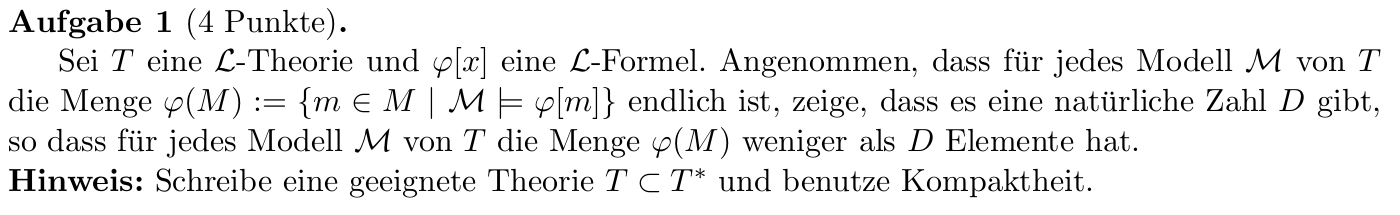
\includegraphics[scale=0.3]{./A-1.png}
        \label{fig:}
    \end{figure}

    \underline{ZZ:} Es gibt ein D $\in \mathds{N}$: Für alle Modelle $\mathcal{M}$ gilt: $|\varphi(M)| < D$\\ 
    \\\underline{Beweis}:\\

    Wir sollen also zeigen, dass in $\mathcal{M}$ nicht gilt $\forall n \in \mathds{N}$:\\
    \\$\varphi_n = \exists x_1,\dots,x_n(\bigwedge_{i \neq j} (\neg x_i \doteq x_j \land \varphi[x_i]))$\\
    \\Das heißt es ist zu zeigen: $T^* = T \cup \{\varphi_n | n \in \mathds{N}\}$ ist widersprüchlich / nicht konsistent\\
    \\Sei $\mathcal{A} \vDash T^*$, dann gilt mit den $\varphi_n$, dass es unendlich viele Belegungen gibt mit $\mathcal{M} \vDash \varphi[x]$\\
    $\Rightarrow \varphi(M)$ ist undendlich groß.\\
    $\Rightarrow T^*$ ist nicht konsistent.\\
    \\$\overset{Kompatkh.}{\Rightarrow}$ eine endliche Teilmenge von $\{\varphi_n | n \in \mathds{N}\}$ ist widersprüchlich.\\
    Also: $\exists n_1,\dots,n_k$ so dass $T \cup \{\varphi_1,\dots,\varphi_k\}$ widersprüchlich.\\
    \\Da $\varphi_n \rightarrow (\bigwedge_{i=1}^n \varphi_i)$ folgt, wenn $m = max(\{n_1, \dots, n_k\})$ ist, dann gilt:\\
    $T \cup \{\varphi_m\}$ ist widersprüchlich.\\
    \\$\overset{Auss.}{\Rightarrow} T \vdash \neg \varphi_m \Rightarrow \forall \mathcal{M}: |\varphi(M)| < m$\\

%}}}

\newpage

\section*{}%{{{
\label{sec:aufgabe_2}

    \begin{figure}[H]
        \centering
        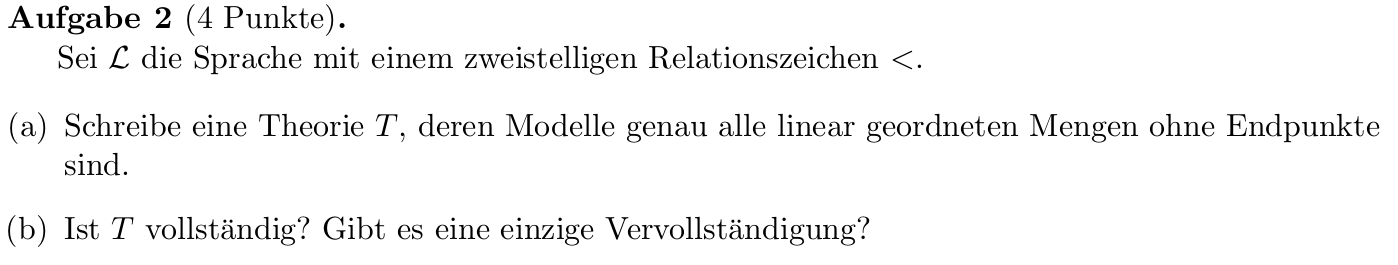
\includegraphics[scale=0.3]{./A-2.png}
        \label{fig:}
    \end{figure}

    \begin{itemize}
        \item a)\\
            Wir schreiben auf welche Eigenschaften wir benötigen und formulieren sie als Aussagen:\\
            \begin{itemize}
                \item Irreflexiv:\\
                    $\forall x \neg x < x$\\
                \item Transitiv:\\
                    $\forall x,y,z ((x < y \land y < z) \rightarrow x < z)$\\
                \item Total:\\
                    $\forall x,y (x < y \lor x \doteq y \lor y < x)$\\
                \item Keine Endpunkte:\\
                    $\forall x \exists y \quad x < y$\\
                    $\forall x \exists y \quad y < x$\\
            \end{itemize}
            T ist dann die Vereinigung aller dieser Aussagen.\\
        \item b)\\
            $R = (\mathds{R}, \{<\}) \text{ und } Z = (\mathds{Z}, \{<\})$ sind offensichtlich Strukturen, die T erfüllen.\\
            Für R gilt jedoch, dass zwischen 2 Zahlen unendlich viele weitere liegen:\\
            \\$\forall x,y \exists z (x < y \rightarrow (x < z \land z < y))$\\
            \\Dies gilt nicht für Z (zwischen 1 und 2 liegt keine ganze Zahl).\\
            Wäre T vollständig müsste entweder die Aussage oder ihre Negation in T gelten.\\
            Da dies offenbar nicht der Fall ist,\\
            wir haben 2 Modelle gefunden in denen jeweils 1 davon gilt,\\
            kann T nicht vollständig sein.\\
    \end{itemize}%}}}

\section*{}%{{{
\label{sec:aufgabe_3}

    \begin{figure}[H]
        \centering
        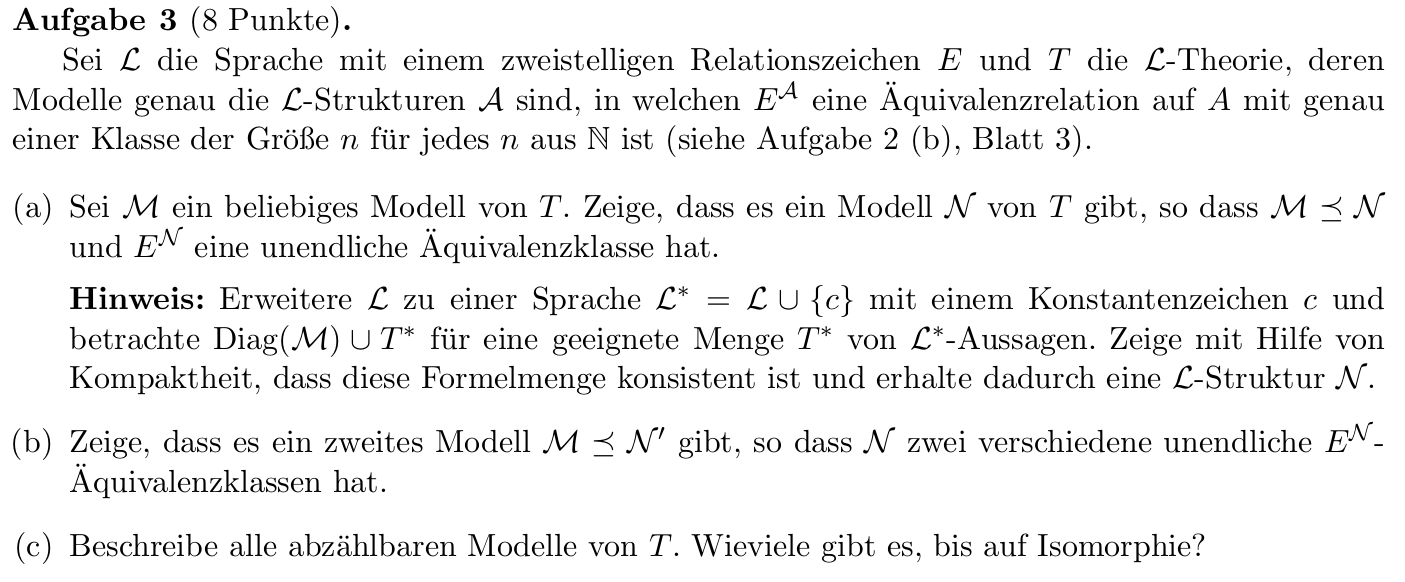
\includegraphics[scale=0.3]{./A-3.png}
        \label{fig:}
    \end{figure}

    \begin{itemize}
        \item a)\\
            \underline{ZZ:} Es gibt ein Modell $\mathcal{M} \preceq \mathcal{N}: E^\mathcal{N}$ hat \underline{eine} undendliche Äquivalenzklasse.\\
            \\\underline{Beweis:}\\ 
            Wir erweitern unsere Sprache nun um ein c, damit wir folgende Aussagen $\varphi_n$ beschreiben können:\\
            $\varphi_n = \exists x_1,\dots,x_n (\bigwedge_{i \neq j} (\neg x_i \doteq x_j \land E(x_i, c)))$\\
            \\Das c soll später also mit unendlich vielen $x_i$ in einer Äquivalenzklasse sein.\\
            Wir beweisen durch Widerspruch, dass ein $\mathcal{N}$ wie in der Aufgabe existiert:\\
            \begin{itemize}
                \item \underline{Annahme:} Diag($\mathcal{M}) \cup \{\varphi_n | n \in \mathds{N}\}$ ist widersprüchlich\\
                    $\overset{Kompatkh.}{\Rightarrow} \exists n_1,\dots,n_k \in \mathds{N}: Diag(\mathds{M}) \cup \{\varphi_n_1,\dots,\varphi_n_k\}$ ist widersprüchlich.\\
                    \\Sei wieder wie in \textcircled{\small{1}} $n = max(\{n_1,\dots,n_k\})$\\
                    $\Rightarrow Diag(\mathcal{M}) \cup \{\varphi_n\}$ ist widersprüchlich.\\
                    \\Sei nun [m] die Äquivalenzklasse mit genau n Elementen und $c^\mathcal{M}^* = m,\\ \text{wobei } \mathcal{M}^* = \mathscr{L}^*(\mathcal{M})$ ist.\\
                    \\$\Rightarrow \mathcal{M}^* \vDash Diag(\mathcal{M}) \cup \{\varphi_n\}$ Widerspruch, da nicht konsistent!\\
            \end{itemize}
            $\Rightarrow Diag(\mathcal{M}) \cup \{\varphi_n | n \in \mathds{N}\}$ ist konsistent.\\
            \\c ist mit unendlich vielen $x_i \in M$ in einer Äquivalenzklasse, damit existiert ein $\mathcal{N}$ wie in der Aufgabe.\\

        \item b)\\
            \underline{ZZ:} Es gibt ein Modell $\mathcal{N}$ für das $E^\mathcal{N}$ genau zwei undendliche Äquivalenzklassen besitzt\\
            \\\underline{Beweis:}\\ 
                Diesmal ist unser $\mathscr{L}^* = \mathscr{L} \cup \{c,d\}$\\
                Wir formulieren jetzt die Anforderungen wieder als Aussagen:\\
                \begin{itemize}
                    \item Es gibt zwei undendliche Äquivalenzklassen:\\
                        $\varphi_n = \exists x_1,\dots,x_n(\bigwedge_{i \neq j} (\neg x_i \doteq x_j \land E(x_i,c)))$\\
                        $\psi_m = \exists x_1,\dots,x_m (\bigwedge_{i \neq j} (\neg x_i \doteq x_j \land E(x_i,d)))$\\
                    \item Diese beiden sind verschieden:\\
                        $\neg E(c,d)$\\
                \end{itemize}
                Dann ist die neue Theorie $T^*:$\\
                $T^* = Diag(\mathcal{M}) \cup \{\varphi_n | n \in \mathds{N}\} \cup \{\psi_m | m \in \mathds{N}\} \cup \{\neg E(c,d)\}$\\
                \\Von hier an geschieht alles analog zu Aaufgabe a)\\

        \item c)\\
            Für alle $n \in \mathds{N}$ gibt es ein Modell mit \underline{genau} n Äquivalenzklassen die unendlich groß sind.\\



    \end{itemize}
%}}}

\newpage

\section*{}%{{{
\label{sec:aufgabe_4}

    \begin{figure}[H]
        \centering
        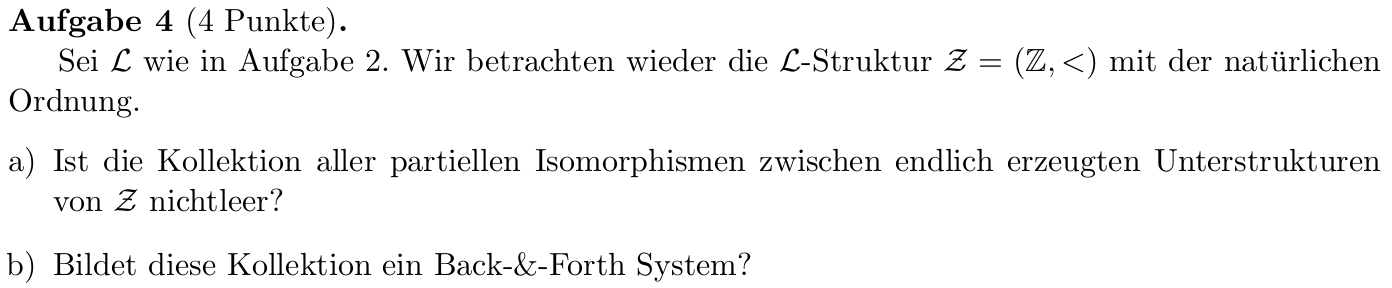
\includegraphics[scale=0.3]{./A-4.png}
        \label{fig:}
    \end{figure}

    \begin{itemize}
        \item a)\\
            \underline{ZZ:} S ist nichtleer.\\
            \\\underline{Beweis:}\\ 
            Sei $\mathcal{A} = (\{1\}, \{<\})$ Struktur (gilt, da < keine Elemente erzeugt).\\
            Dann ist die Abbildung: $\{1\} \rightarrow \{1\}, 1 \mapsto 1$ eine Isomorphie zwischen $\mathcal{A} \text{ und } \mathcal{A}$.
            Da $\mathcal{A}$ offensichtlich endlich erzeugt und Unterstruktur ist, ist S nichtleer.\\

        \item b)\\
            Nein, da wir leicht ein Gegenbeispiel finden können.\\
            \\$\mathcal{A} = (\{1,3\}, \{<\}) \text{ und } \mathcal{B} = (\{1,2\}, \{<\})$ sind endlich erzeugte Unterstrukturen.\\
            \\Aber ist F bereits vorhanden mit $F: \{1,3\} \rightarrow \{1,2\}, F: 1 \mapsto 1, F: 3 \mapsto 2$,\\
            dann kann $\mathcal{A}$ nicht auf A = \{1,2,3\} erweitert werden,\\
            da dann durch 1 < 2 < 3 auch\\
            F(1) < F(2) < F(3) gelten müsste, das ist jedoch 1 < F(2) < 2, es gibt aber kein solches $F(2) \in \mathds{Z}$.\\

    \end{itemize}%}}}
\end{document}
